\documentclass[14pt]{beamer}
\usepackage{hyperref}
\usetheme{boxes}
\usepackage{color}
\usecolortheme{dove}
\usepackage{mathptmx}

\title{Blockchains \& Cryptocurrencies}
\subtitle{Presented to Nairobi Garage}
\author{Evan Klitzke}
\date{January 16, 2018}

\begin{document}

\begin{frame}
  \titlepage
\end{frame}

\AtBeginSection[]
{
  \begin{frame}[plain]{Outline}
    \tableofcontents[currentsection]
  \end{frame}
}

\begin{frame}
\frametitle{Outline}
  \tableofcontents
\end{frame}

\begin{frame}{About Me}
  I am a software engineer based out of San Francisco. I previously worked at
  Google and Uber, now I'm traveling, hacking on crypto stuff, and figuring out
  what's next.
  \newline
  \newline
  I spent most of 2017 working on different crypto projects. In February I'll be
  participating in the \href{https://hackerresidency.com}{Chaincode Residency}
  program in NYC to work on Bitcoin Core.
\end{frame}

\begin{frame}{Slides and Contact Info}
  You can download the slides for this talk at this short link:
  \textbf{\href{https://goo.gl/xUgDSi}{goo.gl/xUgDSi}}
  \newline
  \newline
  The source code for these slides can be found at:
  \href{https://github.com/eklitzke/nairobi-crypto}{github.com/eklitzke/nairobi-crypto}
  \newline
  \newline
  How to reach me in the future:
  \newline
  \newline
  \begin{tabular}{r | l}
    Email & \href{mailto:evan@eklitzke.org}{evan@eklitzke.org} \\
    Web & \href{https://eklitzke.org}{eklitzke.org} \\
    Twitter & \href{https://twitter.com/eklitzke}{@eklitzke} \\
  \end{tabular}
\end{frame}

\section{Bitcoin}

\begin{frame}{Bitcoin Whitepaper}
  The original whitepaper was published by Satoshi Nakamoto on October 31, 2008.
  It can be found here:
  \textbf{\href{https://bitcoin.org/bitcoin.pdf}{bitcoin.org/bitcoin.pdf}}
  \newline
  \newline
  It's very short and accessible: 9 pages total, including a bibliography and
  some sample code. I highly encourage you to read it after this talk.
\end{frame}

\begin{frame}{Who Was Satoshi Nakamoto?}
  Nobody knows.
  \newline
  \newline
  Satoshi mined the first Bitcoin block on January 3, 2009, at the same time he
  released the source code for Bitcoin 0.1.
  \newline
  \newline
  Satoshi was involved with the project until 2010.
  The last code commit from Satoshi was made on August 28, 2010.
\end{frame}

\begin{frame}{Who Controls Bitcoin Today?}
  Today Bitcoin exists as an open source software project on GitHub. There are
  22 people who have the ability to commit new code to Bitcoin (called the
  ``core'' developers).
  \newline
  \newline
  Changes to Bitcoin happen by a process of consensus among the core developers.
  There is no one person or company that controls Bitcoin.
\end{frame}


\begin{frame}{Bitcoin Motivation}
  As explained on the first page of the whitepaper, the motivation is to
  \textbf{``[allow] two willing parties to transact directly with each other
    without the need for a trusted third party''}.
  \newline
  \newline
  In other words: users can send payments to each other without trusting a bank
  (e.g. Kenya Commercial Bank) or a payment processor (e.g. PayPal, Visa, or
  M-PESA).
\end{frame}

\begin{frame}{Secondary Motivations}
  Some of these will be covered in more detail later, but the following are
  additional motivations:

  \begin{itemize}
  \item Reduce transaction fees
  \item Avoid frozen accounts and funds
  \item Avoid transaction reversals
  \item Eliminate trust issues with centralized issuance
  \item Eliminate debasement of currency via inflation
  \end{itemize}
\end{frame}

\begin{frame}{Blockchains}
  As described in the whitepaper, Bitcoin is organized as a \emph{blockchain}.
  \newline
  \newline
  The original idea for blockchains predates Bitcoin by about 10 years. Earlier
  blockchains had serious flaws, which Satoshi solved with Bitcoin.
\end{frame}

\begin{frame}{What Is A Blockchain?}
  At a high level, a blockchain is a linked list of blocks. Blocks are issued on
  some interval (10 minutes for Bitcoin). The blockchain acts as a public ledger
  for all transactions on the network.
  \newline
  \newline
  Each block contains a list of all transactions during that time period. During
  each block interval, one node in the network is selected to create the next
  block via ``proof of work''.
\end{frame}

\begin{frame}{Blockchain Accountability}
  One of the benefits of a blockchain is that all transaction details are part
  of an immutable, public record.
  \newline
  \newline
  All nodes in the network can audit the blockchain to verify that transactions
  are valid, that new money isn't being counterfeited, etc.
\end{frame}

\begin{frame}{Proof of Work}
  The most important idea behind Bitcoin (and other cryptocurrencies) is
  \textbf{proof of work}. This idea actually predates Bitcoin by about a decade.
  \newline
  \newline
  Proof of work is what miners do. We'll spend a few slides on this.
\end{frame}

\begin{frame}{Proof of Work: Properties of Money}
  To be suitable as money, a currency needs to satisfy several properties, among them:
  \newline
  \begin{itemize}
  \item It must be difficult to counterfeit.
  \item Parties should not be able to spend funds they do not have, called the
    ``double spending problem''.
  \end{itemize}
\end{frame}

\begin{frame}{Proof of Work}
  We've known how to avoid double spending for millenia: put all transactions in
  a \emph{ledger}, and check balances at each step.
  \newline
  \newline
  This is improved by double entry bookkeeping, invented in the late 1400's in
  Italy.
\end{frame}

\begin{frame}{Proof of Work: Double Spending}
  To implement a cryptocurrency we need a \emph{distributed} and \emph{decentralized}
  ledger.
  \newline
  \newline
  This is a difficult problem: ledgers must  have \emph{strong consistency}
  with a \emph{well-defined ordering} of transactions.
\end{frame}

\begin{frame}{Proof of Work}
  \textbf{Idea:} Every $N$ minutes, choose one peer in the system at random, and
  let that person create the next block.
  \newline
  \newline
  \textbf{Problem:} How do we choose which person should be selected? How do we ensure it's fair and unbiased?
\end{frame}

\begin{frame}{Proof of Work}
  The idea of \textbf{proof of work} is to come up with a difficult math puzzle
  that takes about $N$ minutes to solve.
  \newline
  \newline
  Whoever solves the puzzle gets to create the next block in the chain.
  \newline
  \newline
  This person is also rewarded with newly issued coins and transaction fees.
\end{frame}

\begin{frame}{Proof of Work: Bitcoin}
  Here's how PoW is implemented in Bitcoin, at a very high level.
  \newline
  \newline
  Each person creates a candidate block and includes a timestamp and
  nonce. The block is hashed twice with a cryptographic hash
  function. If the hash is numerically less than a target difficulty,
  the block is valid, and is accepted by other peers in the network.
\end{frame}

\begin{frame}{Proof of Work: Bitcoin}
  The reason PoW works is that a cryptographic hash function effectively outputs
  a random sequence of zeros and ones.
  \newline
  \newline
  The current Bitcoin difficulty requires about $\mathbf{9.6 \times 10^{21}}$ hashes to find
  a new, valid block. Or in English, about 10 sextillion hashes.
\end{frame}

\begin{frame}{Proof of Work: Bitcoin}
  Proof of Work is \emph{fair} because it's random.
  \newline
  \newline
  The chance of any person mining the next block is proportional to the hashing
  power they provide to the network, and nothing else.
  \newline
  \newline
  Bitcoin hashes block headers, which are \emph{always exactly 80 bytes},
  regardless of the number of transactions in a block.
\end{frame}

\begin{frame}{Counterfeiting}
  The counterfeiting problem is solved by only allowing new coins to be created
  via newly mined blocks.
  \newline
  \newline
  All coins/transactions can be traced to their origin via the blockchain.
\end{frame}

\begin{frame}{Transaction Signatures}
  Transactions are signed and authorized using a digital signature scheme.
  \newline
  \newline
  Currently Bitcoin uses ECDSA signatures. A future release of Bitcoin is likely
  to add support for Schnorr signatures, which are smaller for multisig
  applications.
\end{frame}

\begin{frame}{$M$ of $N$ Signature Schemes}
  ECDSA supports $M$ of $N$ signature schemes using a variant of ElGamal
  signatures. This is often called ``multisig'' in Bitcoin.
  \newline
  \newline
  These can be used to implement things like jointly shared accounts (e.g.
  husband and wife), two factor wallets, funds controlled by a board, etc.
\end{frame}

\begin{frame}{Mining}
  The people who are doing Bitcoin PoW hashing are called ``miners''. When a
  miner finds a new block, they are issued new Bitcoin.
  \newline
  \newline
  The current block reward for Bitcoin (including transaction fees) is worth
  about 15 BTC (20M~Ksh), which is given out about once every 10 minutes.
\end{frame}

\begin{frame}{Non-Reversibility}
  Bitcoin transactions are \textbf{non-reversible}.
  \newline
  \newline
  Unlike ACH, Paypal, or M-PESA, it is impossible to reverse a transaction.
  \newline
  \newline
  This is good for merchants, but users must be more careful about
  fraud/hacking.
\end{frame}

\begin{frame}{Can I Mine Bitcoin?}
  In a word, \textbf{No.}
  \newline
  \newline
  Mining Bitcoin requires very specialized hardware, and access to extremely
  cheap power.
\end{frame}

\begin{frame}{Tracking Balances}
  Bitcoin uses unspent transaction outputs (UTXOs), which are fairly complex,
  but give Bitcoin pseudononymity.
  \newline
  \newline
  Most other cryptocurrencies use simpler accounting systems, which typically
  sacrifice anonymity.
\end{frame}

\begin{frame}{Anonymity}
  Bitcoin is considered to be ``pseudonymous'', meaning that transactions are
  tied to Bitcoin addresses, but addresses are not associated with individuals.
  \newline
  \newline
  If \emph{used properly}, Bitcoin is relatively anonymous, especially compared
  to most other cryptocurrencies.
\end{frame}

\begin{frame}{Inflation}
  Most governments have a central bank that issues new notes, which debases the
  currency via inflation.
  \newline
  \newline
  The inflation rate in Kenya between 2005 and 2017 averaged 10\%.
  \newline
  \newline
  The official inflation rate in the USA (CPI-U) is about 2\%, but it's likely
  closer to 6\% (due to changes the Fed made in 1990 for measuring the CPI).
\end{frame}

\begin{frame}{Bitcoin Is Not Inflationary}
  Bitcoin is non-inflationary, and issuance happens at a \emph{decreasing pace}.
  \newline
  \newline
  At most \textbf{21M} Bitcoins will ever be created. So far 16.8M
  Bitcoins have been mined (about 80\% of all Bitcoins).
  \newline
  \newline
  Because issuance is decreasing while adoption is increasing,
  Bitcoin is effectively deflationary: the value of Bitcoin is increasing over
  time.
\end{frame}

\begin{frame}{Bitcoin Issuance}
  \begin{figure}
    %\input{supply}
    \resizebox{\columnwidth}{!}{\input{supply}}
  \end{figure}
\end{frame}

\begin{frame}{Bitcoin Problems}
  Recently, the Bitcoin network has reached maximum capacity, and is running
  into scaling problems.
  \newline
  \newline
  This has led to very high transaction fees---on the order of thousands of Ksh
  per transaction. This has partly helped the rise of other cryptocurrencies,
  which attempt different solutions to this problem.
\end{frame}

\begin{frame}{Lightning Network}
  The most exciting development upcoming in Bitcoin is the Lightning Network
  (LN). This enables \emph{off-chain scaling} of Bitcoin.
  \newline
  \newline
  A bunch of complicated math and cryptography allows two parties to create a
  payment channel that allows them to securely transact Bitcoin without using
  the main Bitcoin network.
  \newline
  \newline
  LN should be available for mainstream use this year.
\end{frame}

\begin{frame}{Review}
  No person or company controls Bitcoin: it is truly open and distributed.
  \newline
  \newline
  Bitcoin is:
  \begin{itemize}
  \item A distributed, open source project.
  \item Secure, and can be easily audited.
  \item Non-inflationary, or even deflationary.
  \item Relatively anonymous.
  \item Not a fad: it's more than nine years old!
  \end{itemize}
\end{frame}

\section{Ethereum}

\begin{frame}{Ethereum}
  The second most popular cryptocurrency after Bitcoin is called Ethereum.
  \newline
  \newline
  The most important way that Ethereum differs from Bitcoin is through
  \textbf{smart contracts}.
  \newline
  \newline
  This year Ethereum will also begin testing \textbf{proof of stake} as an
  alternative to proof of work.
\end{frame}

\begin{frame}{History}
  \begin{itemize}
  \item The project was first proposed by Vitalik Buterin in late 2013
  \item A crowdsale took place in mid-2014 to fund the project
  \item The project went line in mid-2015
  \end{itemize}
\end{frame}

\begin{frame}{The Ethereum Virtual Machine}
  The main idea behind Ethereum was to create a brand new cryptocurrency that
  implemented a universal, distributed ``virtual machine''.
  \newline
  \newline
  The EVM allows programmers to create immutable ``smart contracts'' that
  interact with the Ethereum network.
\end{frame}

\begin{frame}{Smart Contracts}
  Smart contracts are usually written in a high level language like Solidity
  (based on Javascript) that compile to EVM code.
  \newline
  \newline
  Smart contracts are \textbf{immutable}: once put on the Ethereum network, they
  can never change. This has upsides, and downsides.
\end{frame}

\begin{frame}{Cryptokitties}
  \makebox[\textwidth]{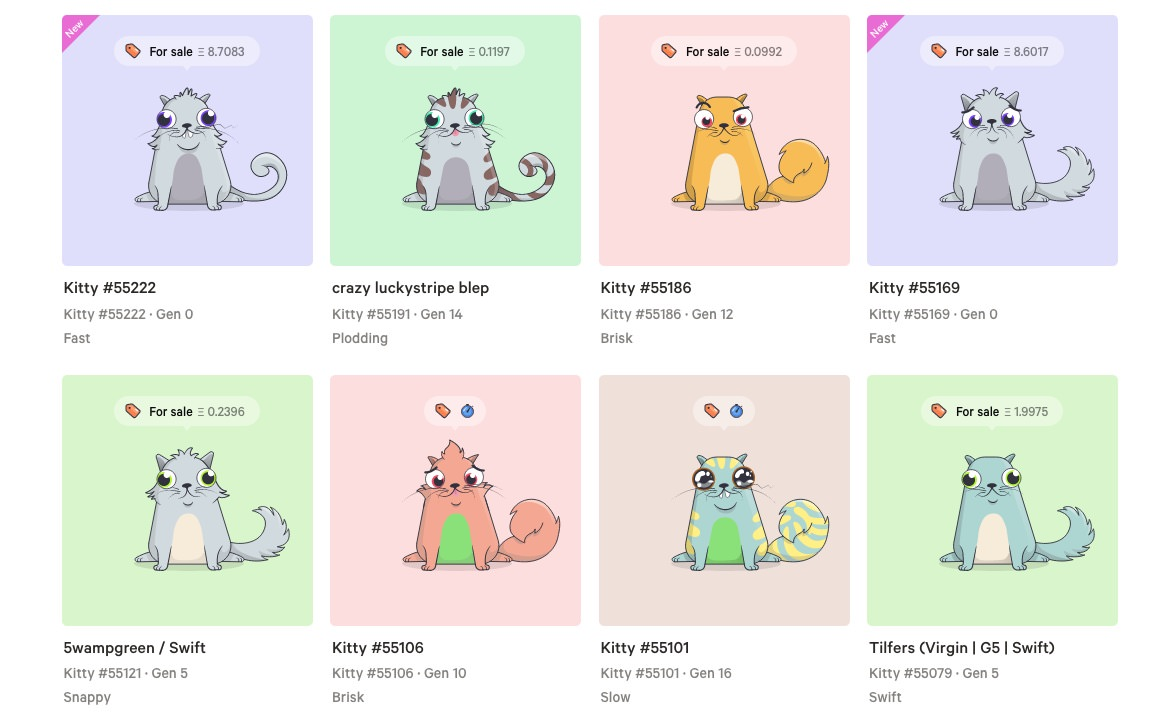
\includegraphics[scale=0.25]{cryptokitties.jpg}}
\end{frame}

\begin{frame}{Proof of Stake}
  The idea of proof of stake (PoS) is that instead of giving new coins to miners, new
  coins should be given to existing holders of coins.
  \newline
  \newline
  The primary motivation is to reduce ``wasted'' electricity caused by mining.
\end{frame}

\begin{frame}{PoS Caveats}
  Hashing is still needed to secure the network, so by necessity PoS will exist
  alongside conventional PoW mining.
  \newline
  \newline
  This is an active research area, and there is a lot of debate about how to
  best implement PoS and its implications. Hence the Ethereum team is moving
  somewhat slowly (and cautiously) on this.
\end{frame}

\begin{frame}{ERC20 Tokens}
  Ethereum has a standardized way to create new coins based on Ethereum, called
  \textbf{ERC20 Tokens}.
  \newline
  \newline
  For instance, I can easily create a new token called \emph{EvanCoin} that has a
  limited supply and some other minor changes to Ethereum.
\end{frame}

\begin{frame}{Bitsoko}
  Bitsoko (\href{https://bitsoko.co.ke}{bitsoko.co.ke}) is a local Nairobi
  startup that is working with Ethereum to provide various services to local
  businesses and merchants.
  \newline
  \newline
  One of these services is a system to help local companies issue ERC20 tokens
  as a funding mechanism for their business.
\end{frame}

\section{Other Coins}

\begin{frame}{Other Coins}
  In this section I'll talk briefly about a few other cryptocurrencies,
  sometimes called ``altcoins'':

  \begin{itemize}
  \item Litecoin
  \item Bitcoin Cash
  \item Monero
  %\item Ripple
  \end{itemize}
\end{frame}

\begin{frame}{Litecoin}
  Litecoin is one of the oldest altcoins. It's a fork of Bitcoin that just changes a few parameters:
  \newline
  \begin{itemize}
  \item Block interval is shortened by $1 / 4$ (from 10 minutes to 2.5 minutes)
  \item Coin supply is increased by $4 \times$ (from 21M to 84M)
  \end{itemize}
  Recently, Litecoin has morphed into a testbed for new ideas that may be
  integrated into Bitcoin.
\end{frame}

\begin{frame}{Bitcoin Cash}
  Bitcoin Cash is a fork of Bitcoin that increases the block size, with the goal
  of lowering transaction fees.
  \newline
  \newline
  This fork is extremely divisive within the Bitcoin community.
  \newline
  \newline
  If you decide to purchase Bitcoin, know if you are buying real Bitcoin, or
  Bitcoin Cash.
\end{frame}

\begin{frame}{Monero}
  Monero is applying novel ideas in cryptography to create a \emph{completely
    anonymous} cryptocurrency.
  \newline
  \newline
  Monero obscures:
  \begin{itemize}
  \item Who payments are going to/from
  \item How much money is being transacted in payments
  \item The balance on accounts
  \end{itemize}
\end{frame}

%% \begin{frame}{Ripple}
%%   Ripple is a \emph{centralized} cryptocurrency created by a for-profit company,
%%   that has been popular recently due to its price.
%%   \newline
%%   \newline
%%   Ripple claims that banks are using their token for inter-bank transfers, but
%%   so far this mostly seems to be marketing/hype.
%% \end{frame}

\section{Private Blockchains}

\begin{frame}{Private Blockchains}
  Private blockchains are an alternative to decentralized cryptocurrencies like
  Bitcoin and Ethereum.
  \newline
  \newline
  In a private blockchain, a central authority has the ability to issue new
  tokens, destroy tokens, reverse transactions, etc.
\end{frame}

\begin{frame}{Efficiency}
  One advantage of private blockchains is they tend to be drastically more
  efficient and scalable than distributed blockchains.
  \newline
  \newline
  Private blockchains do not use proof of work or mining. The central authority
  issuing coins signs new blocks using a set of private keys they control.
\end{frame}

\begin{frame}{Example: Royal Mint Gold}
  The UK Royal Mint recently launched RMG (``royal mint gold'') as a way to
  digitize gold held in the Royal Mint's bank vaults.
  \newline
  \newline
  The Royal mint can issue new RMG tokens if they add gold to their vaults, and
  likewise they can destroy tokens if they remove gold from their vaults.
\end{frame}

\begin{frame}{Other Use Cases}
  People have proposed using private blockchains for many applications, e.g.:
  \begin{itemize}
  \item Energy credits
  \item Digitizing other physical assets (e.g. barrels of oil)
  \item Deeds or land sales
  \end{itemize}
  \end{frame}

\begin{frame}{Utility of Private Blockchains}
  Private blockchains are attractive because they offer third parties more
  visibility and transparency compared to traditional databases.
  \newline
  \newline
  However, traditional databases are still simpler and scale better than private
  blockchains.
  \newline
  \newline
  It's unclear if private/centralized blockchains have long term viability.
\end{frame}

\section{Exchanges}

\begin{frame}{Crypto Exchanges}
  Services that let you trade or purchase cryptocurrencies are called exchanges.
  \newline
  \newline
  Some exchanges only allow trading between cryptocurrencies. Others allow
  purchasing cryptocurrencies with ``fiat'' currency.
\end{frame}

\begin{frame}{Kenyan Exchanges}
  Most exchanges are localized to a specific country for practical reasons: the
  relevant laws vary greatly from country to country.
  \newline
  \newline
  I cannot endorse any Kenyan exchanges specifically, but I saw a few when
  searching Google.
\end{frame}

\begin{frame}{Local Bitcoins \& Local Ethereum}
  You can also purchase Bitcoin or Ethereum directly from another person using a
  service like LocalBitcoins or LocalEthereum.
  \newline
  \newline
  You will see a list of people in Kenya willing to sell Bitcoin/Ethereum. Most
  sellers I saw here will trade for M-PESA.
\end{frame}

\begin{frame}{Risks of Exchanges}
  If purchase Bitcoin (or Ethereum) on an exchange and leave it there, there's a
  risk that if the exchange (or your account) is hacked, you will lose your
  money.
  \newline
  \newline
  Be careful with your crypto! I will tell the story of Mt. Gox and BTC-e
  later in this talk.
\end{frame}

\section{Initial Coin Offerings (ICOs)}

\begin{frame}{ICOs}
  ICOs (``initial coin offerings'') were originally created to fund development
  for new cryptocurrency projects.
  \newline
  \newline
  For example, the Ethereum developers did a crowdsale where they sold 2000 ETH
  for 1 BTC.
  \newline
  \newline
  The BTC they raised was used to finance development of Ethereum,
  which launched about a year later.
\end{frame}

\begin{frame}{Recent Developments}
  ICOs have become an extremely popular way to raise large amounts of capital,
  bypassing the normal venture capital or investment banking system.
  \newline
  \newline
  Multiple American and European startups launched ICOs that raised more than
  \$100M (10B Ksh), which has led to many copycat ICOs.
\end{frame}

\begin{frame}{The ICO Cycle}
  The reason ICOs have been able to raise so much capital is tied to the ability
  of investors to later sell their ICO tokens on exchanges at a profit.
  \newline
  \newline
  Many investors have an expectation that their tokens will be listed on
  cryptocurrency exchanges, where they can be resold at a premium.
\end{frame}

\begin{frame}{Regulatory Status}
  In the USA, the sale of \textbf{equities} is regulated by the SEC. SEC rules
  require that only \emph{accredited investors} can purchase equity from pre-IPO
  companies.
  \newline
  \newline
  To quality as an accredited investor, one must have a net worth of \$1,000,000
  (100B Ksh) excluding one's primary residence, or continued earnings of at
  least \$200,000 (20M Ksh) per year.
\end{frame}

\begin{frame}{Recent Developments}
  The SEC has recently started cracking down on ICOs, if the tokens sold appear
  to qualify as equities under US law.
  \newline
  \newline
  There has also been pressure on exchanges not to list these tokens, as only
  tokens that are listed on exchanges can easily be sold at a profit.
\end{frame}

\begin{frame}{ICO Scams}
  In some cases, the people behind ICOs have either literally disappeared with
  the money they raised (e.g. Confido, FMtokens).
  \newline
  \newline
  In other cases, the companies behind the ICOs have completely failed to
  actually deliver a product (e.g.~Tezos).
\end{frame}

\begin{frame}{Good ICOs}
  Not all ICOs are bad: if done in a responsible way, an ICO can be a powerful
  tool for entrepreneurs to raise money for an idea. Ethereum is an example of
  an ICO success story, done in a responsible way.
  \newline
  \newline
  It's important for investors to be wary and skeptical of ICOs they're
  considering investing in, and it's important for entrepreneurs to do ICOs in a
  responsible and legal way.
\end{frame}

\begin{frame}{Advice For Investors}
  Investors should ask themselves:
  \begin{itemize}
  \item How much money is this company trying to raise?
    \item What utility do the tokens have? Are they valuable for anything other
      than flipping?
    \item Who is behind the ICO? What is their track record?
    \item What does the distribution of tokens look like? How much are the
      investors keeping for themselves?
  \end{itemize}
\end{frame}

\begin{frame}{Advice For Businesses}
  Businesses considering ICOs should be responsible, and comply with existing
  regulations.
  \newline
  \newline
  Future legislation regarding ICOs and crypto tokens will be based on what's
  happening in the market today.
  \newline
  \newline
  The long term viability of ICOs and crypto
  tokens is predicated on responsible actions by entrepreneurs launching ICOs.
\end{frame}

\section{Other Regulatory Issues}

\begin{frame}{Legality}
  As a \emph{user}, you just need to know that cryptocurrencies are legal, and
  are technically considered to be \textbf{assets} rather than money.
  \newline
  \newline
  As a \emph{business}, you should know that many things in this area are
  operating in a \textbf{legal gray area}, as there are few or no laws
  specifically regulating cryptocurrencies.
\end{frame}

\begin{frame}{For Users}
  If you make a profit buying and selling cryptocurrencies, you must report
  those earnings and pay taxes on your capital gains (5\% in Kenya).
  \newline
  \newline
  This isn't really crypto-specific, the same would be true if you sold your
  Pok\'{e}mon cards or vinyl record collection.
\end{frame}

\begin{frame}{For Businesses}
  As a business, you can probably \emph{accept} Bitcoin/Ethereum payments
  without concern---just make sure you pay the taxman.
  \newline
  \newline
  Things are much more complicated if you want to offer exchange-like services,
  e.g. if you wanted to create a business that let people buy Bitcoin with Ksh.
\end{frame}

\begin{frame}{FATF}
  International money transmission is tightly regulated by international
  agreements, particularly FATF (a.k.a. GAFI).
  \newline
  \newline
  FATF has the objectives of combating:
  \begin{itemize}
    \item International money laundering.
    \item Terrorism financing.
  \end{itemize}
\end{frame}

\begin{frame}{KYC \& AML Laws}
  KYC (``know your customer'') laws require that institutions offering banking
  services know who their customers are. Typically this means collecting
  suitable ID for new clients.
  \newline
  \newline
  AML (``anti-money laundering'') laws require that institutions offering
  banking services need to take certain steps to ensure they're not aiding money
  laundering.
\end{frame}

\section{Blockchain Ideas For Africa}

\begin{frame}{Banking The Unbanked}
  It's estimated that two thirds of people in Sub-Saharan Africa are
  unbanked\footnote{For some definition of ``unbanked''}. Sending money across
  borders (or even within countries) is still unreliable and expensive in many
  parts of Africa.
  \newline
  \newline
  This is not just an African problem: only 27\% of adults in Southeast Asia are
  thought to have a bank account.
\end{frame}

\begin{frame}{Banking The Unbanked}
  Many countries with large unbanked populations also suffer from high rates of
  inflation.
  \newline
  \newline
  Is it possible to help unbanked people using cryptocurrencies or
  blockchains?
\end{frame}

\begin{frame}{E2E Verifiable Voting}
  The same cryptography underpinning blockchains and cryptocurrencies can be
  used in end-to-end verifiable voting schemes.
  \newline
  \newline
  Ballots cast are put into a public ledger, which anyone can verify.
\end{frame}

\begin{frame}{E2E Verifiable Voting}
  Voters get a receipt after voting.
  \newline
  \newline
  Voters can verify that their vote was actually counted, by checking that it
  actually appears in the public ledger.
\end{frame}

\begin{frame}{E2E Verifiable Voting}
  Here's where things get weird.
  \newline
  \newline
  Although voters can confirm that their vote was counted, and that it was cast
  for the right person, \textbf{other people cannot tell from the receipt who the
    voter voted for}.
  \newline
  \newline
  This prevents politicians from paying for votes (since they can't tell from
  the receipt if a vote was cast for them), and prevents physical intimidation
  when voters exit voting stations.
\end{frame}

\begin{frame}{E2E Verifiable Voting}
  There are a lot of different variations of E2E voting systems, but none of
  them have progressed very far outside of academic circles.
  \newline
  \newline
  Most people are inherently distrustful of voting systems already, and
  electronic voting systems more so.
  \newline
  \newline
  The main obstacle here is likely convincing people who are not expert
  cryptographers that E2E voting systems really are secure, verifiable, and an
  improvement over traditional ballots.
\end{frame}

\section{Q{\&}A}

\begin{frame}{Q{\&}A}
  Now is the time to ask questions!
  \vspace{10mm}
  \newline
  \begin{tabular}{r | l}
    Slides & \href{https://goo.gl/xUgDSi}{goo.gl/xUgDSi} \\
    Email & \href{mailto:evan@eklitzke.org}{evan@eklitzke.org} \\
    Web & \href{https://eklitzke.org}{eklitzke.org} \\
    Twitter & \href{https://twitter.com/eklitzke}{@eklitzke} \\
  \end{tabular}
\end{frame}

\end{document}
